%---------------------------------------------------------------------------------------------------
%		virtualization.tex
%
%	This is the main file of the chapter that talk about the paas layer of SPI.
%
%	Author: Andrea Meneghinello
% Version: 0.1
%	Table of changes:
%		18/03/2016 -> document definition
%---------------------------------------------------------------------------------------------------
\section{Virtualization}
\label{sec:background-virtualization}
Both \ac{paas} and \ac{iaas} layer of \ac{spi} model are provided through virtualization techniques.
Even if cloud computing can be provided without using virtualization technologies, they allow to
reduce operative and capital costs.

With the term \keyword{virtualization} we refer to the act of creating a virtual version of something,
including, but not limited, to a virtual computer hardware platform, \acs{os}es, storage devices or
network resources. Thus we can assert that virtualization is an isomorphism\footnote{Isomorphism is
a term that derive from the mathematics	domain and refers to a bijective application between objects
from different set.} between the virtual system, known as \keyword{guest}, and real one known as
\keyword{host}.

Through virtualization we want to provide high levels of performance and also gain in scalability,
reliability, availability and also in agility. Virtualization provides us an artificial view of the
physical world, on which many resources are viewed as single one or the opposite (one resource
is viewed as many individuals). Furthermore it can make a single large storage resource appear to be much
smaller or the opposite (many storage devices can appear as a big single device). It is also able to group
related processes together without making them able to see processes of other groups.

In this area virtualization provides a virtual version of a computer system, known with the name of
\keyword{\ac{vm}}. \citeauthor{vmArchitecture} in \cite{vmArchitecture} define \ac{vm} as:

\begin{quote}
	``a component that provides a complete, persistent system environment that support an \acs{os}
	along with its many users's processes. It provides the guest operating system which access to
	virtual hardware resources including networking, I/O, \ac{gui} along with processors and memory.''
\end{quote}

Virtualizing physical infrastructures helps to improve their scalability and their utilization. It is 
important to notice that it also enables the \acs{it} personnel to perform administration tasks in an
easier way. In the next section we will do a brief digression about the \ac{iaas} model and analyse
which assets are provided the other \ac{spi} models.

\subsection{Assets for cloud computing}
\label{sec:background-virtualization-assets}
As we asserted in the precedent section, \ac{paas} is possible only because \ac{iaas} model exists.
To correctly support other \ac{spi} models it must provide them the following assets:

\begin{itemize}
	\item{\keyword{computing}: means executing users' tasks with the appropriate compute capacity. It is
		able to aggregate multiple computational resources to provide more power, or sharing the available
		resources in order to support tasks coming from different users. Anyway it must ensure
		\keyword{isolation}, \keyword{security} and \keyword{fast scalability};}
	\item{\keyword{storage}: means hiding physical storage devices, their location and their sharing between
		multiple users. Storage virtualization provides the following features: \ac{dfs},
		artificial storage volumes, arrays of storage volumes, a greater control over the available space and
		finally that different architecture can share the same storage devices;}
	\item{\keyword{networking}: means hiding the real complexity of the network by separating (or aggregating)
		the overall network system into manageable parts. Usually network virtualization provides the 
		following features: routing, \ac{nat}, isolation and aggregation.}
\end{itemize}

\subsection{Virtualization types}
\label{sec:background-virtualization-types}
There exists two type of virtualization and they differ for the level in which they offer it; they
are: \keyword{hardware level virtualization} (virtualize over \ac{isa}) and \keyword{\acs{os} level
virtualization} (virtualize over \ac{abi} level). In this thesis we are mostly interested in \acs{os}
level virtualization; Further analysis about the first one can be found in \citeauthor{gardimanThesis}'s
master thesis \cite{gardimanThesis}.
Figure \ref{img:background-paas-virtualization-assets-virtualizationLevels}
shows a generic computer architecture and highlights the possible level of virtualization.

\begin{figure}
	\centering{}
	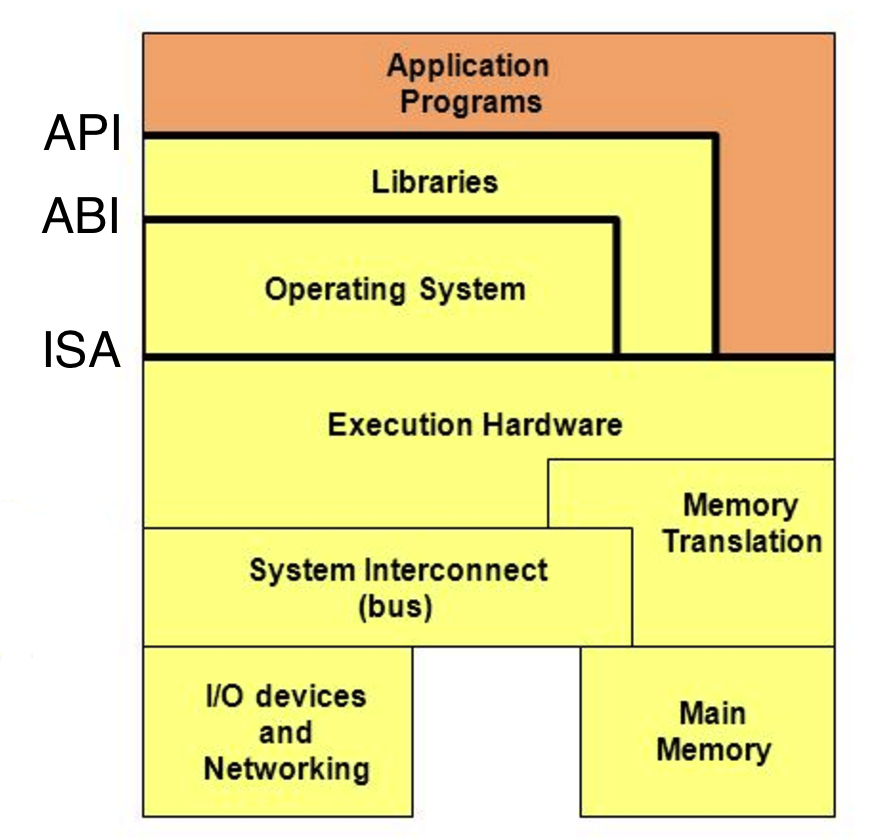
\includegraphics[width=0.5\textwidth]{chapters/background/images/computing-virtualization.png}
	\caption[Different computing virtualization levels]{Overview of computer architecture that shows at
		which layer we can provide virtualization. \acf{iaas} allow virtualization over \acf{isa}, instead
		\ac{paas} provide virtualization over \acf{abi} and finally \ac{saas} allows virtualization over
		\ac{api} \cite{virtualizationLevel}.}
	\label{img:background-paas-virtualization-assets-virtualizationLevels}
\end{figure}

To be thorough, we are going to spend some words about hardware level virtualization in order to correctly
understand the difference with the other type. At Hardware level the virtualization isomorphism is managed
by a software layer called \keyword{hypervisor}, which can be of two different types (shown in Figure 
\ref{img:background-paas-virtualization-assets-virtualizationTypes}):

\begin{itemize}
	\item{\keyword{native} (type 1): a native hypervisor runs directly over the physical hardware ensuring
		a complete control of the same. In this case the hypervisor must be compatible with all the physical
		hardware thus being able to manage it;}
	\item{\keyword{hosted} (type 2): a hosted hypervisor runs over an host \acs{os} which lies above the
		physical architecture; this topology delegates to the host \acs{os} the following tasks: hardware
		drivers management, available memory management, resources allocation management and finally process
		scheduling.}
\end{itemize}

The hosted hypervisor can produce a reduction of the perceived performance because of the presence of a 
further layer that the native type does not have. As a consequence a system, call originated by an 
application or service inside one \ac{vm}, needs more time to reach the underlying hardware downgrading 
the general performance.

\begin{figure}
	\centering{}
	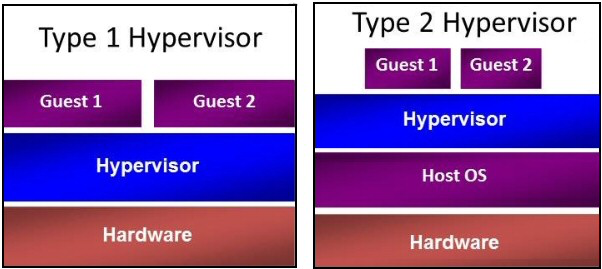
\includegraphics[width=0.6\textwidth]{chapters/background/images/virtualization-types.png}
	\caption[Virtualization types]{The stack generated by the two different type of virtualization.
		We can see the native (type 1) on the left and hosted one (type 2) on the right
		\cite{virtualizationTypes}.}
	\label{img:background-paas-virtualization-assets-virtualizationTypes}
\end{figure}

The hypervisor can virtualize the underlying hardware using three different approaches:

\begin{itemize}
	\item{\keyword{full-virtualization}: the hypervisor completely virtualizes the underlying hardware,
		ensuring a full compatibility with any \acs{os} that supports the physical infrastructure;}
	\item{\keyword{hardware-assisted virtualization}: the hypervisor is built as an extension of the
		previous one (full-virtualization). In this case the processor has a built-in architectural support
		that facilitate the forward phase, to the underlying hardware, of a system call generated by an
		application or service that runs inside a \ac{vm};}
	\item{\keyword{para-virtualization}: hypervisor does not offer an interface that simulates the
		underlying hardware but exposes a modified one to \ac{vm}s (closer the real one), called Virtual
		Hardware \acs{api}, explicitly designed for the \ac{vm}s; an advantage of this type of virtualization
		is that it is possible to implement an interface agnostic to the underlying hardware; instead
		the major weakness is that in case of a system crash all the current \ac{vm}s will be affected by
		the problem.}
\end{itemize}

Unlike hardware level virtualization, \acs{os}-virtualization  provides a virtual view over the
\ac{abi}. In this case the guest and the host share same \acs{os} and host hardware.

Users' processes execute on the host and they are (as much as possible) isolated from each other.
Logical separated environments are called \keyword{containers}.
Figure \ref{img:background-paas-virtualization-assets-virtualizationTypeDifference} shows the
difference between \acs{os} level virtualization and hardware level one.

Containers technology has existed for a long time. Examples of containers that runs outside Linux
ecosystem are Solaris Zones \cite{solarisContainers}, and \acs{bsd} jails \cite{bsdContainers}.
Instead containers' technology for the Linux ecosystem are: Linux-Vserver \cite{vserverContainers}
and OpenVZ \cite{openvzContainers}. Even though all these technologies have matured, they did not make
significant progress in order to create a proper standard technology.

The containers landscape changed when Linux containers reached a level of maturity that lead them 
into the mainstream Linux kernel with the project \keyword{\ac{lxc}}. This last one uses mainly two
kind of Linux kernel features: \keyword{namespaces} and \keyword{cgroups}.

\begin{figure}[h!]
	\centering{}
	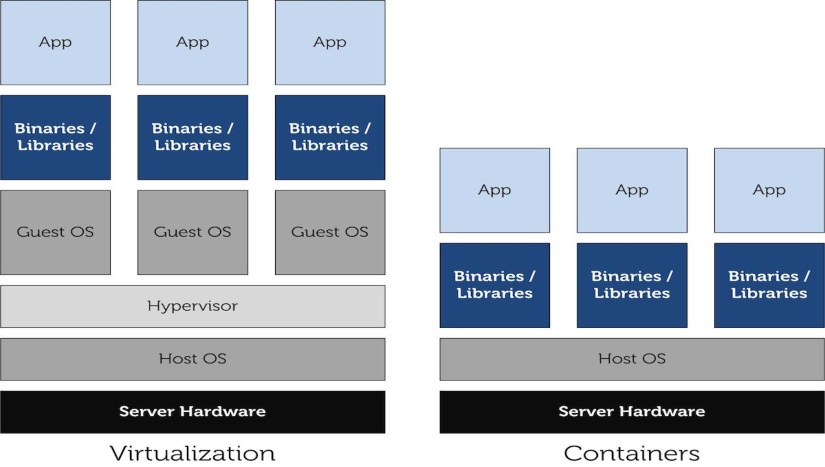
\includegraphics[width=0.7\textwidth]{chapters/background/images/containerization.png}
	\caption[Difference from containerization and virtualization]{Difference from the generated stack
		by hardware level virtualization (type 2) and containerization.}
	\label{img:background-paas-virtualization-assets-virtualizationTypeDifference}
\end{figure}

The namespace is able to isolate processes resources though the following namespaces:

\begin{itemize}
	\item{PID: processes residing in a namespace cannot affect others namespace's processes. This
		means that processes inside a container are not able to see or alter processes that reside in
		another container;}
	\item{NET: each net-namespace have a different, and isolated view of the network interfaces. Each
		one has its own routing-table, iptable chains and rules;}
	\item{IPC: each process can communicate only with processes that are in the same \ac{ipc} group. This
		is necessary to maintain process isolation;}
	\item{MNT: processes that live in different mnt-namespace can see other sets of mounted \ac{fs} and
		root directories. If a \ac{fs} is mounted in an mnt-namespace, it will be accessible only to those
		that are in the same namespace;}
	\item{UTS: it is able to give containers a different host-name.}
\end{itemize}

Instead cgroups is able, through a set of rules, to measure and limit the resource consumption on which
containers have access.

\ac{lxc} is a good technology that allows users to run several applications isolated from each other. It
is able to assure an amount of resource capacity to each container. However, even with this feature,
Linux containers have never reached a wide level of adoption because of their lack in handiness. Everything
has changed when a company named ``docCloud'' delivered an open-source project called \keyword{Docker}.
We will deep about Docker and its architecture in Section \ref{sec:background-docker}.

\subsection[\acs{kvm}]{\acf{kvm}}
\label{sec:background-virtualization-kvm}
\ac{kvm} is a Linux feature that allows Linux to act as a type 1\footnote{See Section
\ref{sec:background-virtualization-types} for additional information about type 1 and type 2.} hypervisor
running an unmodified guest \acs{os} inside a Linux process. \ac{kvm} uses hardware virtualization features
in recent processors to reduce complexity and overhead.

\ac{kvm} supports both emulated \acs{io} devices (through \ac{qemu}) and paravirtual \acs{io} devices
(through virtio). The combination of hardware acceleration and paravirtual \acs{io} is designed with
the aim to reduce the virtualization overhead to very low levels \cite{mcdougall2010virtualization}.
\ac{kvm} is also able to support ``live migrations'' which permit to hardware engineers to evacuate
some or all servers inside a data-centre for maintenance without disrupting the guest \acs{os}.

Since a \ac{vm} has a static number of virtual-\acs{cpu}s and a fixed amount of \acs{ram}, its resource
consumption is bounded. A single virtual-\acs{cpu} cannot use more than one real \acs{cpu} and each page
of virtual-\acs{ram} maps to at most one page of physical pages in physical \acs{ram} (plus the nested page
table). \ac{kvm} can resize \ac{vm}s while they are running through ``hotplugging'' and ``ballooning''
of v\acs{cpu} and v\acs{ram}, although these techniques require support from the guest \acs{os} and it
is rarely used in real cloud platforms.

Because each \ac{vm} is a process, all normal Linux resource management facilities, like scheduling and
cgroupgs (see Section \ref{sec:background-virtualization-types}) apply to \ac{vm}s. This simplifies the
implementation and administration of the hypervisor but complicates resource management inside the guest
\acs{os}.

\acs{os}s generally assume that \acs{cpu}s are always running and the physical memory has relatively
fixed access times, but under \ac{kvm} v\acs{cpu}s can be unscheduled without notification and v\acs{ram} can
be swapped out, causing performance anomalies that can be hard to debug. \ac{vm}s also have two level
of allocation and scheduling: one in the hypervisor and one in the host \acs{os}. Many cloud providers
eliminate those problems by not overcommitting resources, pinning each v\acs{cpu} to a physical one,
and locking all v\acs{ram} into real \acs{ram}. These techniques essentially eliminate scheduling
activities inside the hypervisor. Moreover fixed resource allocation also simplifies the billing
phase.

\ac{vm}s naturally provide a certain level of isolation and security because of their narrow interface;
the only way a \ac{vm} can communicate with the outside world is through a limited number of hyper-calls
or emulated devices, both of which are controlled by the hypervisor. This is not a panacea, since a few
hypervisor privilege escalation vulnerabilities have been discovered and they could allow a guest \acs{os}
to ``break out'' of its \ac{vm} ``sandbox''.

While \ac{vm} excel at isolation, they add overhead when sharing data between guests or between guest
and hypervisor. Usually such sharing requires fairly expensive marshalling and hyper-calls. In the
cloud, \ac{vm}s generally access storage through emulated block devices backed by image files; creating,
updating and deploying such disk images can be time-consuming and collections of disk images with
mostly-duplicate contents can waste storage space.

\subsection{Main characteristics}
\label{sec:background-virtualization-characteristics}
Virtualization has three main characteristics: partitioning, isolation and encapsulation.

\keyword{Partitioning} refers to the fact that many applications and \acs{os}es are supported in a single 
physical system by separating (partitioning) the available resources. \keyword{Isolation} refers to the
fact that each \ac{vm} is isolated from its physical system and other \ac{vm}; because of isolation, if
one virtual instance crashes it does not affect the others\footnote{Except in case of para-virtualization.}
and data are not shared between different \ac{vm}s\footnote{If data sharing between \ac{vm}s is a requirement
it must be implemented as a software feature.}. Finally \keyword{encapsulation} property derives from
the fact that \ac{vm}s are represented (and even stored) as a single file, hence system administrators
can identify them easily based on the service that they provide.

From the cited properties we can affirm that cloud computing and Virtualization are not interchangeable
because they approach the \acs{it} goals from different perspectives: virtualization has the aim to
isolate computing resources in order to make possible the change of underlying layers without worrying
about higher levels; instead cloud computing has the ability to make computing resources available on
demand providing us the pay-per-use paradigm.